
\begin{equation}
    p' = f(r) e^{i(m \theta + k x - \omega t)}
\end{equation}
Recall thaT the mode is of the 
form 
\begin{equation}
    e^{i k_x x}
    \label{eqn:fluctuationexample}
\end{equation}
if $k_x$ has a real part, $k_{x,real}$ and an imaginary part $i k_{x,imag}$ 
then,

\begin{align}
    &= e^{i k_x x} \\
    &= e^{i (k_{x,real}+ i k_{x,imag}) x} \\
    &= \underbrace{e^{i k_{x,real}x}}_{\textit{amplitude}} \underbrace{e^{- k_{x,imag} x}}_{\textit{exponential decay}} 
\end{align}

Although the ``cut-off'' decay to nearly zero rapidly, the rate at which this occured
was not much of a concern earlier on in turbomachinery design. As nacelles 
continue to grow shorter, a mode that is ``cut-off'' may make it outside the duct.

For this work a desired amplitude was arbitrarily chosen for a mode, $y_{desired}$
and then the axial location at which this occurred, $x_{desired}$ which 
can be compared against a desired length for a nacelle.  
Since SWIRL assumes an infinitely long duct, there is nothing limiting the 
modes propagation with respect to nacelle length. For example, if the 
desired amplitude is one percent, then $x_{desired}$ is $0.46$, 

\begin{align*}
    0.01 &=  e^{-10 x_{desired}},\\
    -\frac{ln|0.01|}{10} &=  x_{desired},\\
    -\frac{ln|0.01|}{10} &= 0.4605170185988091 .
\end{align*}


 \begin{figure}
     \centering
     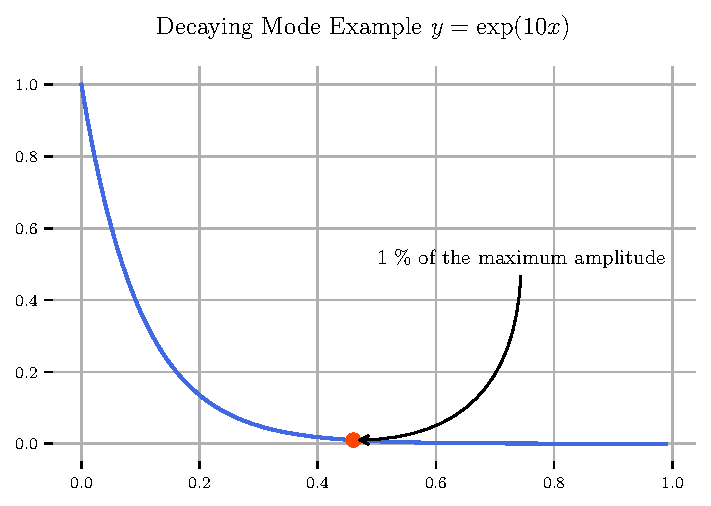
\includegraphics[width=\textwidth]{/home/jeff-severino/SWIRL/CodeRun/04-plotReport/tex-outputs/desired_cut_off_location_1_percent_of_max.pdf}
     \caption{Decaying mode with $k_x = 0 + 10j$ and unit amplitude. One percent
     of the maximum amplitude is identified for nacelle length comparison}
     \label{fig:decaying_mode_with_1_percent_amp}
 \end{figure}
 
 
In general,
\begin{align*}
    y_{desired} &=  e^{-k_{x,imag} x_{desired} }\\
    -\frac{ln|y_{desired}|}{k_{x,imag}} &=  x_{desired}
\end{align*}
